\chapter{Math}
\label{chap:math}

%in the end: sort sections in order of reference in work


\section{Correlations}
\label{sec:correlations}

auto correlation

cross correlation\\
Pearson linear correlation\\
Spearman rank correlation

Correlation in Linear Regression: \url{http://www.stat.yale.edu/Courses/1997-98/101/correl.htm}\\


\section{Lognormal distribution}
\label{sec:lognormal_distribution}

This is a small summary about the lognormal probability distribution \citep[p.~780]{Bronstein2000}. The lognormal distribution is the distribution of a random variable $X$ if the logarithm of $X$ conforms to a normal distribution. Its shape is highly asymmetric, however in a semi-log plot the Gaussian bell curve is recognizable (see the second panel of \autoref{fig:lognormal_3panel_pdfcairo_plot}).
\begin{figure}[htb]
	%\centering
	\fcapside[\FBwidth]{
		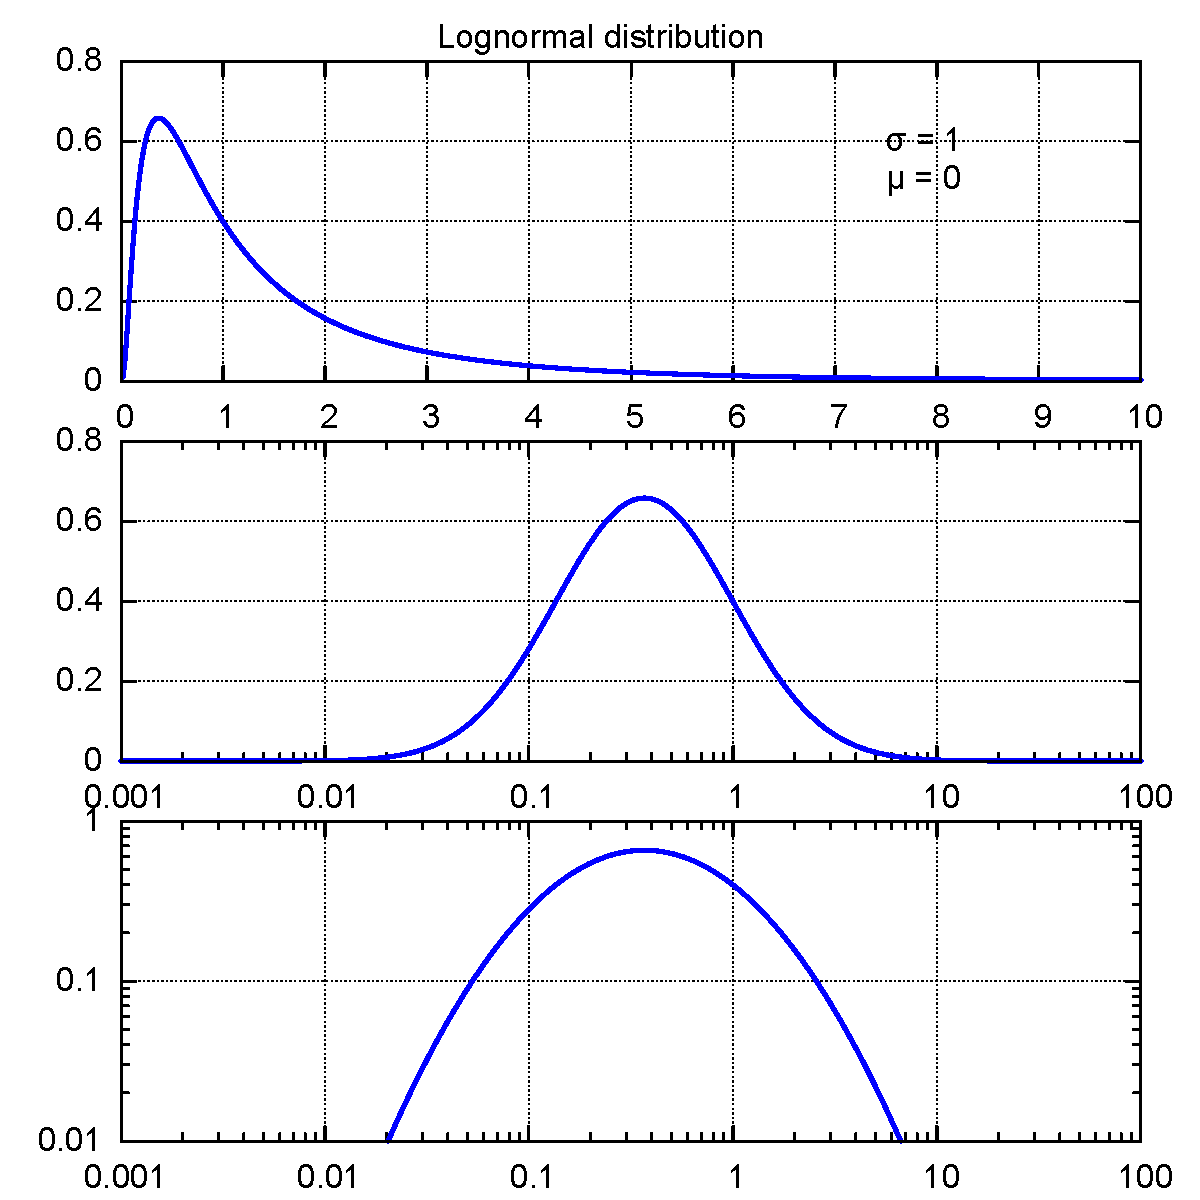
\includegraphics[width=0.5\textwidth]{images/gnuplots/lognormal_3panel_pdfcairo_plot.pdf}
	}{
		\caption{The lognormal probability density function ($\sigma = 1, \mu = 0$) plotted in a linear, semi-log and log-log way.}
		\label{fig:lognormal_3panel_pdfcairo_plot}
	}
\end{figure}
Its probability density function is
\begin{align}
	f(x) &= \frac{1}{\sigma \sqrt{2 \pi} x} \, \text{e}^{- \frac{(\ln x - \mu)^2}{2 \sigma^2}}
\end{align}
with the location ($\mu$) and the shape parameter ($\sigma$). Changes in $\mu$ affect both the horizontal and vertical scaling of the function, whereas $\sigma$ has an influence on its shape (see \autoref{fig:lognormal_ms_pdfcairo_plot}).\\
\begin{figure}[htb]
	\centering
	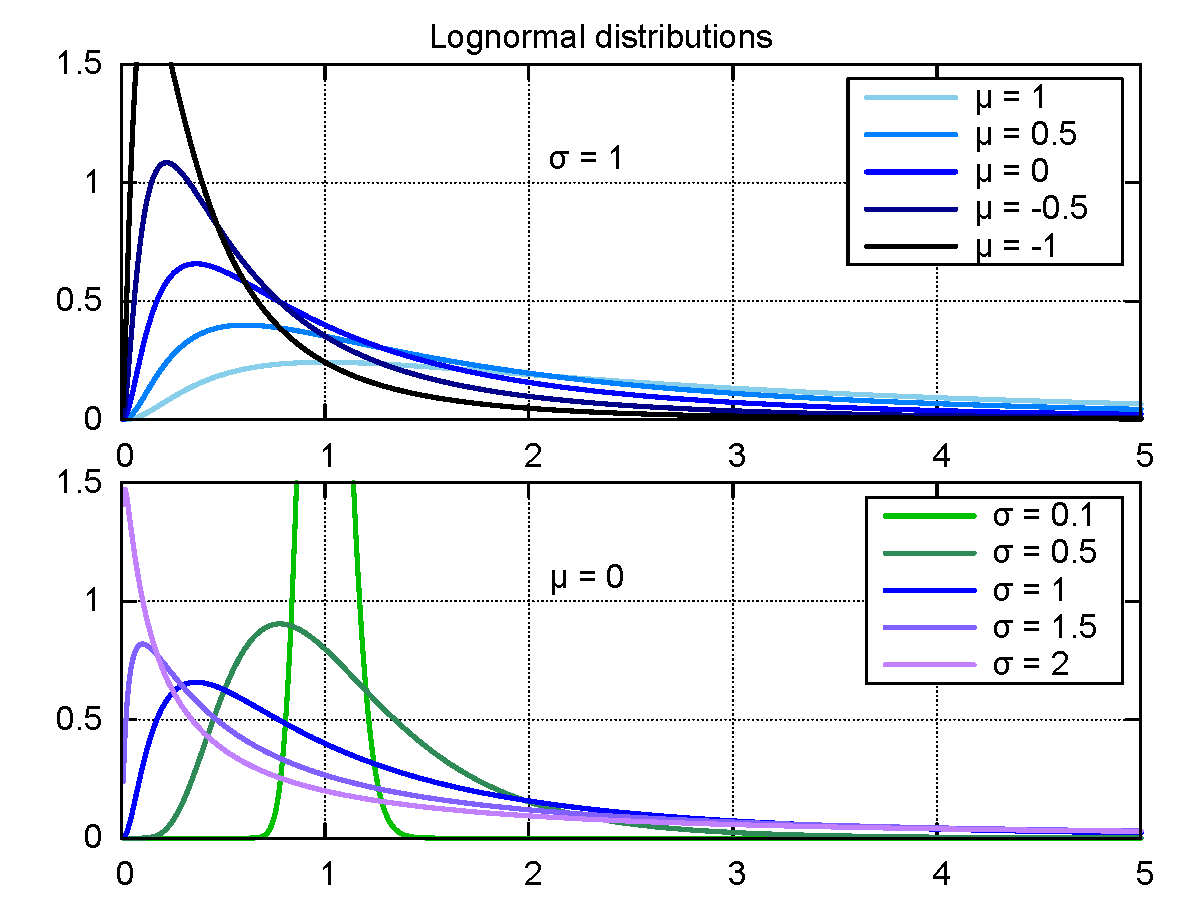
\includegraphics[width=0.5\textwidth]{images/gnuplots/lognormal_ms_pdfcairo_plot.pdf}
	\caption{Five lognormal distributions plotted with fixed $\sigma$ (top) and fixed $\mu$ (bottom).}
	\label{fig:lognormal_ms_pdfcairo_plot}
\end{figure}

Because it is a probability distribution, its area is normalized
\begin{align}
	\int_0^\infty f(x) \text{d} x = 1\,.
\end{align}

For a lognormally distributed random variable the geometric moments mean, standard deviation and variance are:
\begin{align*}
	&\mu_\text{g} = \text{e}^\mu ,\\
	&\sigma_\text{g} = \text{e}^\sigma ,\\
	&var_\text{g} = \text{e}^{\sigma^2}~~(!) .
\end{align*}

Its arithmetic moments are:
\begin{align*}
	&\mu_\text{a} = \text{e}^{\mu + \frac{\sigma^2}{2}} ,\\
	&\sigma_\text{a} = \text{e}^{\mu + \frac{\sigma^2}{2}} \, \left(\text{e}^{\sigma^2} - 1\right) ,\\
	&var_\text{a} = \sigma_\text{a}^2 .
\end{align*}

Other useful characteristics are the median and the mode
\begin{align*}
	&x_\text{median} = \text{e}^{\mu},\\
	&x_\text{mode} = \text{e}^{\mu - \sigma^2}\,.
\end{align*}
Note that for the lognormal distribution its median is equal to its geometric mean.\\

Applications of lognormal distributions...\\
%Limpert2001: Lognormal Distributions across the Sciences: Keys and Clues
%http://bioscience.oxfordjournals.org/content/51/5/341.full

Most natural quantities which can only be positive are lognormally distributed. e.g. animal body sizes?, animal life expectancies, financial stock prices...; income distributions.\\

%life expectancy analyses of economic, technical and biological processes. Bronstein2000


\section{Goodness of fit}
\label{sec:goodness_of_fit}

%figure with fit residuals here
$SSR$ -- sum of squared residuals\\
\begin{align}
	SSR = \sum_i (y_i - f_i)^2
\end{align}
data values $y_i$, fit function values $f_i$\\
$SSR_\text{red}$ -- reduced SSR, divided by number of degrees of freedom $\nu$\\
\begin{align}
	SSR_\text{red} = \frac{SSR}{\nu}
\end{align}
$TSS$ -- total sum of squares (in relation to the data mean)\\
\begin{align}
	TSS = \sum_i (y_i - \bar{y})^2
\end{align}
with data mean $\bar{y}$\\
%http://math.stackexchange.com/questions/1225103/whats-in-a-name-sum-of-squares
%https://en.wikipedia.org/wiki/Goodness_of_fit

$\chi^2$ -- chi-square\\
$\chi^2_\text{red}$ -- reduced chi-square, divided by number of degrees of freedom $\nu$\\

$R^2$ -- coefficient of determination\\
$0 \leq R^2 \leq 1$, ``values can be less than zero''!. if $R^2 = 1$ -> ideal fit; if $R^2 = 0$ -> bad fit
\begin{align}
	R^2 &= 1 - \frac{SSR}{TSS}
\end{align}
``In case of a single regressor, fitted by least squares, R2 is the square of the Pearson product-moment correlation coefficient relating the regressor and the response variable.'' cite from wikipedia \\%https://en.wikipedia.org/wiki/Coefficient_of_determination
%https://de.wikipedia.org/wiki/Bestimmtheitsma%C3%9F

Kolmogorov-Smirnov K-S-Test
%http://www.physics.csbsju.edu/stats/KS-test.html
%http://www.wessa.net/rwasp_Reddy-Moores%20K-S%20Test.wasp


\section{other}

%minimum variance analysis
minimum variance analysis (MVA)\\
determining magnetic cloud configuration \citep{Bothmer1998}\\

hodogramm?
%https://en.wikipedia.org/wiki/Hodograph



least-squares fit approximates mean
linear regression

robust statistics

Non-parametric inferential statistical methods are mathematical procedures for statistical hypothesis testing which make no assumptions about the probability distributions of the variables being assessed. The most frequently used tests include
- median
- percentiles (quartiles)
- Spearman's rank correlation coefficient

histogram

generalized mean
\url{http://en.wikipedia.org/wiki/Generalized_mean}



normal distribution

% inverse erf
% http://mathworld.wolfram.com/InverseErf.html
% 
% \begin{align}
% 	erfc^{-1}(x) = erf^{-1}(1 - x)
% \end{align}
% 
% quantile function: inverse cumulative distribution function (CDF) of normal distribution
% \begin{align}
% 	\mu - \sqrt{2}*\sigma*erfc^{-1}(2*x)
% \end{align}
% http://www.wolframalpha.com/input/?i=Quantile+function+normal+distribution

